% Created 2016-05-01 Son 13:54
\documentclass[11pt, a4paper]{article}
\usepackage[utf8]{inputenc}
\usepackage[T1]{fontenc}
\usepackage{fixltx2e}
\usepackage{graphicx}
\usepackage{longtable}
\usepackage{float}
\usepackage{wrapfig}
\usepackage{soul}
\usepackage{textcomp}
\usepackage{marvosym}
\usepackage{wasysym}
\usepackage{latexsym}
\usepackage{amssymb}
\usepackage{hyperref}
\tolerance=1000
\usepackage{minted}
\usepackage[utf8]{inputenc}
\usepackage[english]{babel}
\usepackage{graphicx}
\usepackage[left=2.35cm, right=3.35cm, top=3.35cm, bottom=3.0cm]{geometry}
\usepackage{titling}
\providecommand{\alert}[1]{\textbf{#1}}

\title{Statistical methods for bioinformatics \linebreak Gene expression: case study (de Vijver et al.)}
\author{Cedric Lood}
\date{\today}
\hypersetup{
  pdfkeywords={},
  pdfsubject={},
  pdfcreator={Emacs Org-mode version 7.9.3f}}

\begin{document}

\maketitle


\graphicspath{ {figures/} }
\setlength{\droptitle}{-5em} 
\setlength{\parindent}{0cm}

\section{Dataset exploration}
\label{sec-1}

The dataset under consideration consists of values of about 5000 gene
expressions (obtained through a microarray technology) for 188
patients. Some of the patients developed distant metastases while some
did not, and the goal is to see if we can use the information from the
levels of gene expressions to predict the metatstases phenotype.

One thing to note from the dimensions of the dataset is that we are
falling in the case of so-called high dimensionality with a number of
observations $n$ that is over an order of magnitude lower than that of
predictors $p$. Among other things, this prevents the use of least
square methods, common in linear models. 

One of the risk when trying to come up with a gene panel that would
predict the evolution of the cancer is that high levels of colinearity
between the predictors likely exists. This renders the set of gene
selected contingent on the particular analysis performed.
\section{Predictive potential}
\label{sec-2}

Here are the libraries I used for this part, and the dataset:

\begin{minted}[]{R}
library(glmnet)
library(polycor)
library(ROCR)
library(leaps)

load("VIJVER.Rdata")
\end{minted}

As a first approach, I tried to search systematically through the
dataset for variables that would correlate with the binary outcome
with a correlation score above 0.45 (for a score of 0.5, the procedure
returns only 2 results).


\begin{minted}[]{R}
## Systematic identification of correlated genex/outcome
genes <- character()
i <- 1
for(gene in names(data)[2:length(data)]) {
    if(abs(hetcor(data$meta, data[gene])$correlations[1,2]) > 0.45){
        genes[i] <- gene
        i <- i + 1
    }
}
\end{minted}

Here is the list of genes returned:


\begin{verbatim}
 [1] "NM_000987"      "NM_003258"      "NM_003295"      "NM_004119"     
 [5] "NM_004203"      "NM_002808"      "NM_002811"      "NM_012291"     
 [9] "NM_013277"      "NM_003981"      "NM_004701"      "M96577"        
[13] "NM_007019"      "NM_007057"      "NM_007267"      "NM_007274"     
[17] "NM_006607"      "NM_016185"      "Contig48913_RC" "NM_018410"     
[21] "NM_001168"      "NM_002106"
\end{verbatim}

Which I then used to build a logistic model, with a best subset
selection approach. For the selection, I used the BIC metric to
select the subset of variable (see graphic)


\begin{minted}[]{R}
## Use the identified variables to create a model
regfit.full <- regsubsets(data.meta~., reduced.data, nvmax = length(genes))
reg.summary <- summary(regfit.full)

## fitting model with the 4 params
reg <- glm(meta~NM_000987+NM_003258+NM_004119+NM_002811, data=data,family = binomial(link=logit))
summary(reg)
reg.probs <- predict(reg, type="response")
contrasts(data$meta)
table(data$meta, fitted(reg)>0.5)
predict <- fitted(reg)
pred <- prediction(predict, data$meta)
perf <- performance(pred, measure="tpr", x.measure = "fpr")
performance(pred, measure="auc")

## using bic to make a decision, n=4
which.min(reg.summary$bic)
coef(regfit.full,4)

## plotting the results
pdf("bic-auc.pdf", width = 16, height = 8)
par(mfrow = c(1,2))
plot(reg.summary$bic, ylab="bic", type="l")
plot(perf, col="red")
dev.off()
\end{minted}

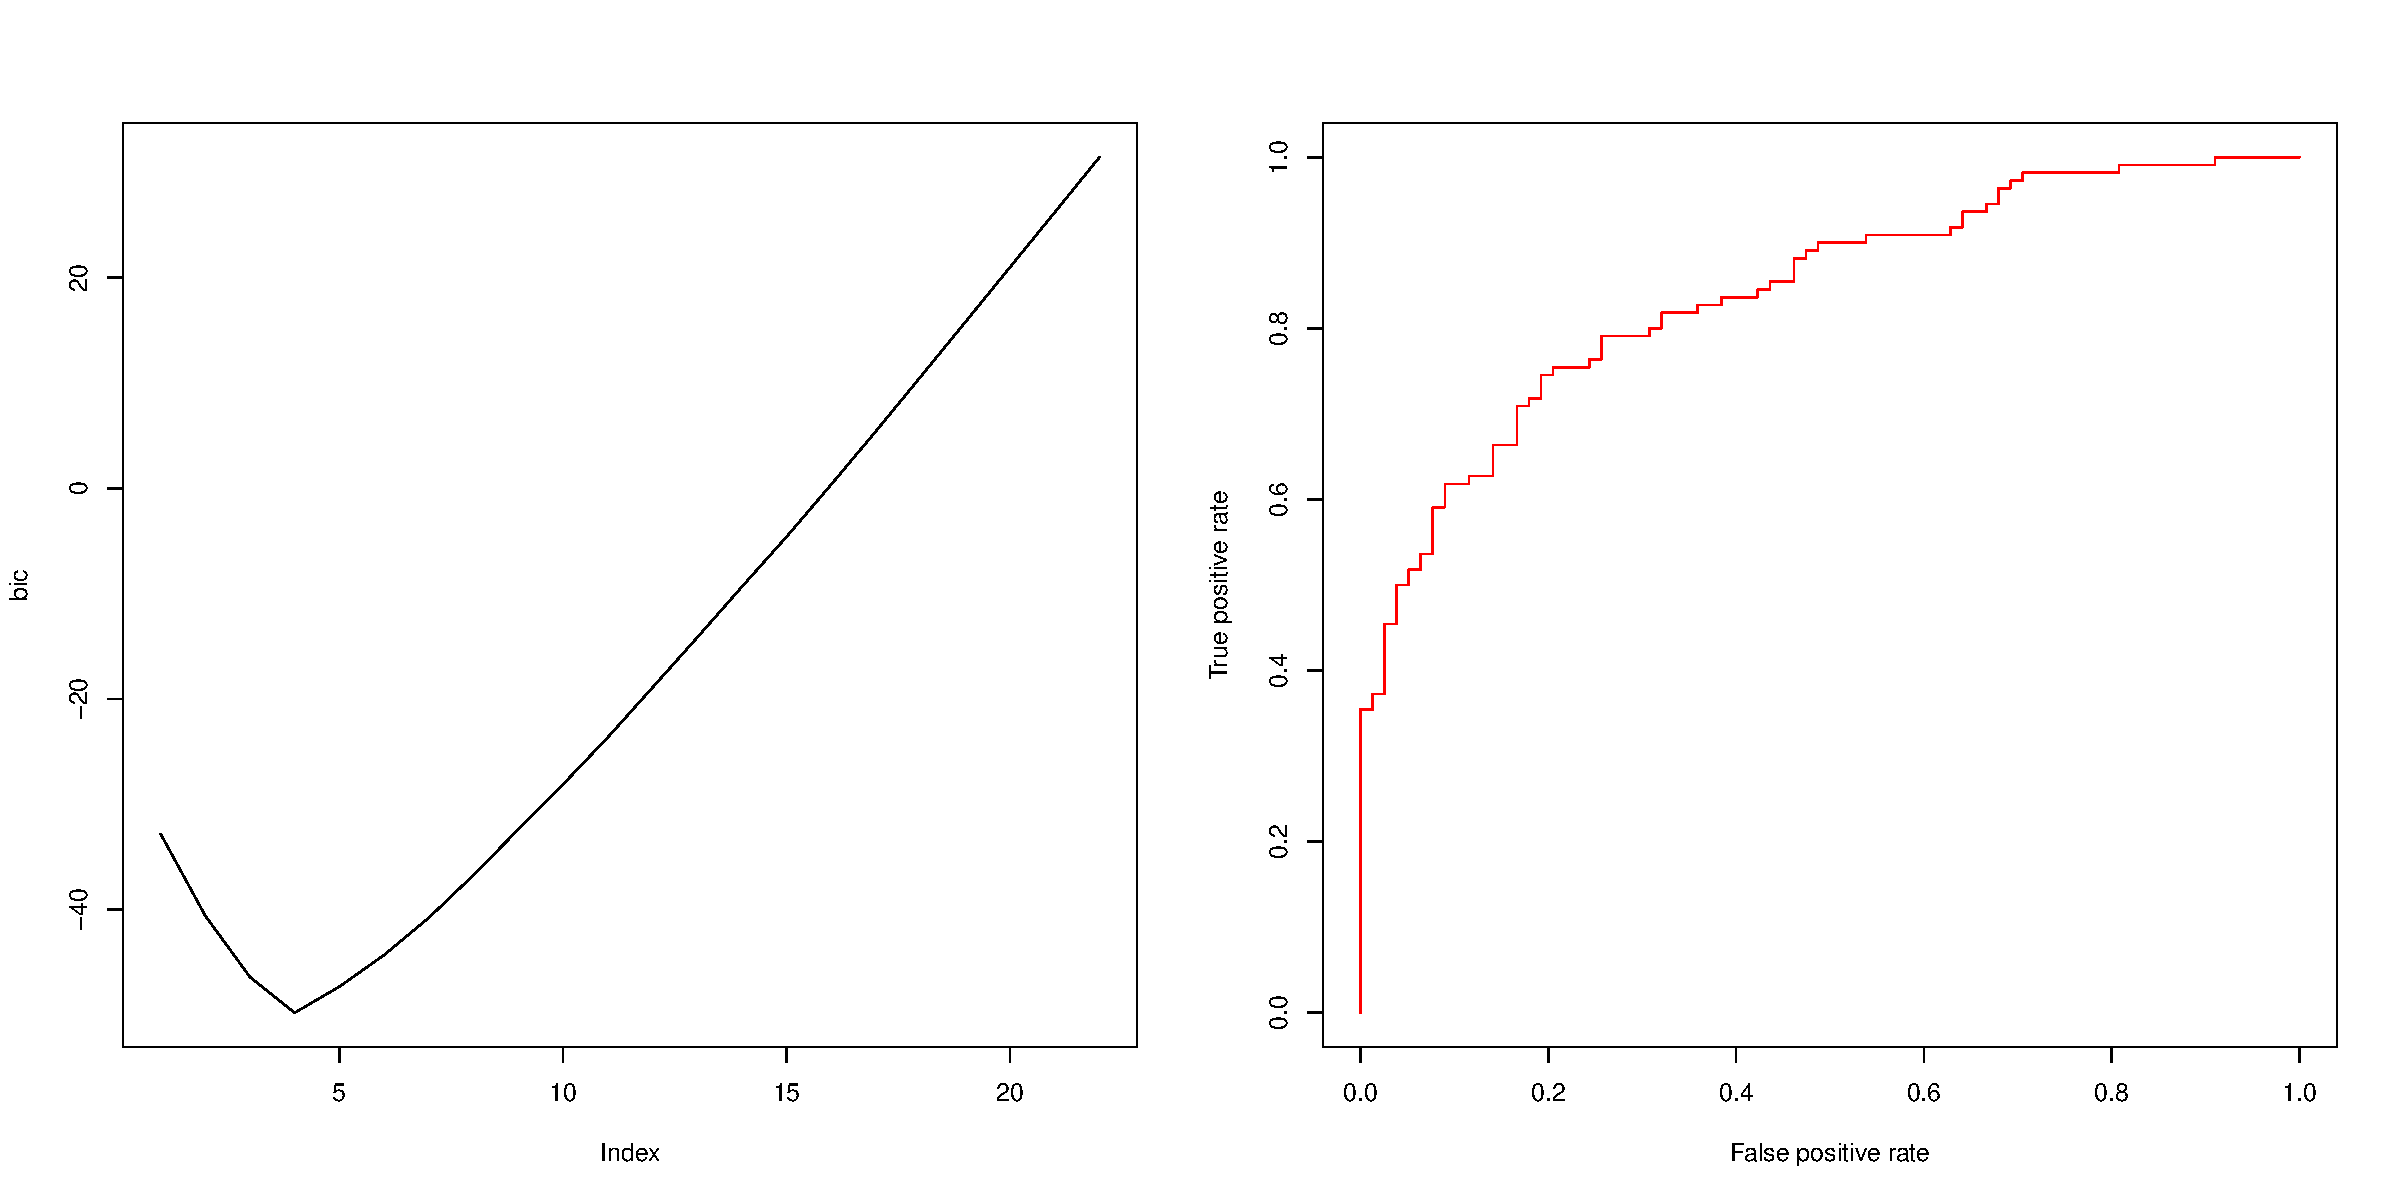
\includegraphics[scale=0.4]{bic-auc.pdf}
\section{Collinearity structure}
\label{sec-3}

Given the size and the nature of the data collected (RNA expression),
we can certainly expect colinearity between different
transcripts. Working with the reduced dataset of 22 transcript levels
created above, one can alreay show multiple examples of such
colinearity:


\begin{minted}[]{R}
pairs(reduced.data[,2:8])
cor(reduced.data$NM_002808,reduced.data$NM_002811)
pairs(reduced.data[,9:16])
cor(reduced.data$NM_003981,reduced.data$NM_004701)
\end{minted}


\begin{verbatim}
> cor(reduced.data$NM_002808,reduced.data$NM_002811)
[1] 0.5072933
> cor(reduced.data$NM_003981,reduced.data$NM_004701)
[1] 0.8694202
\end{verbatim}


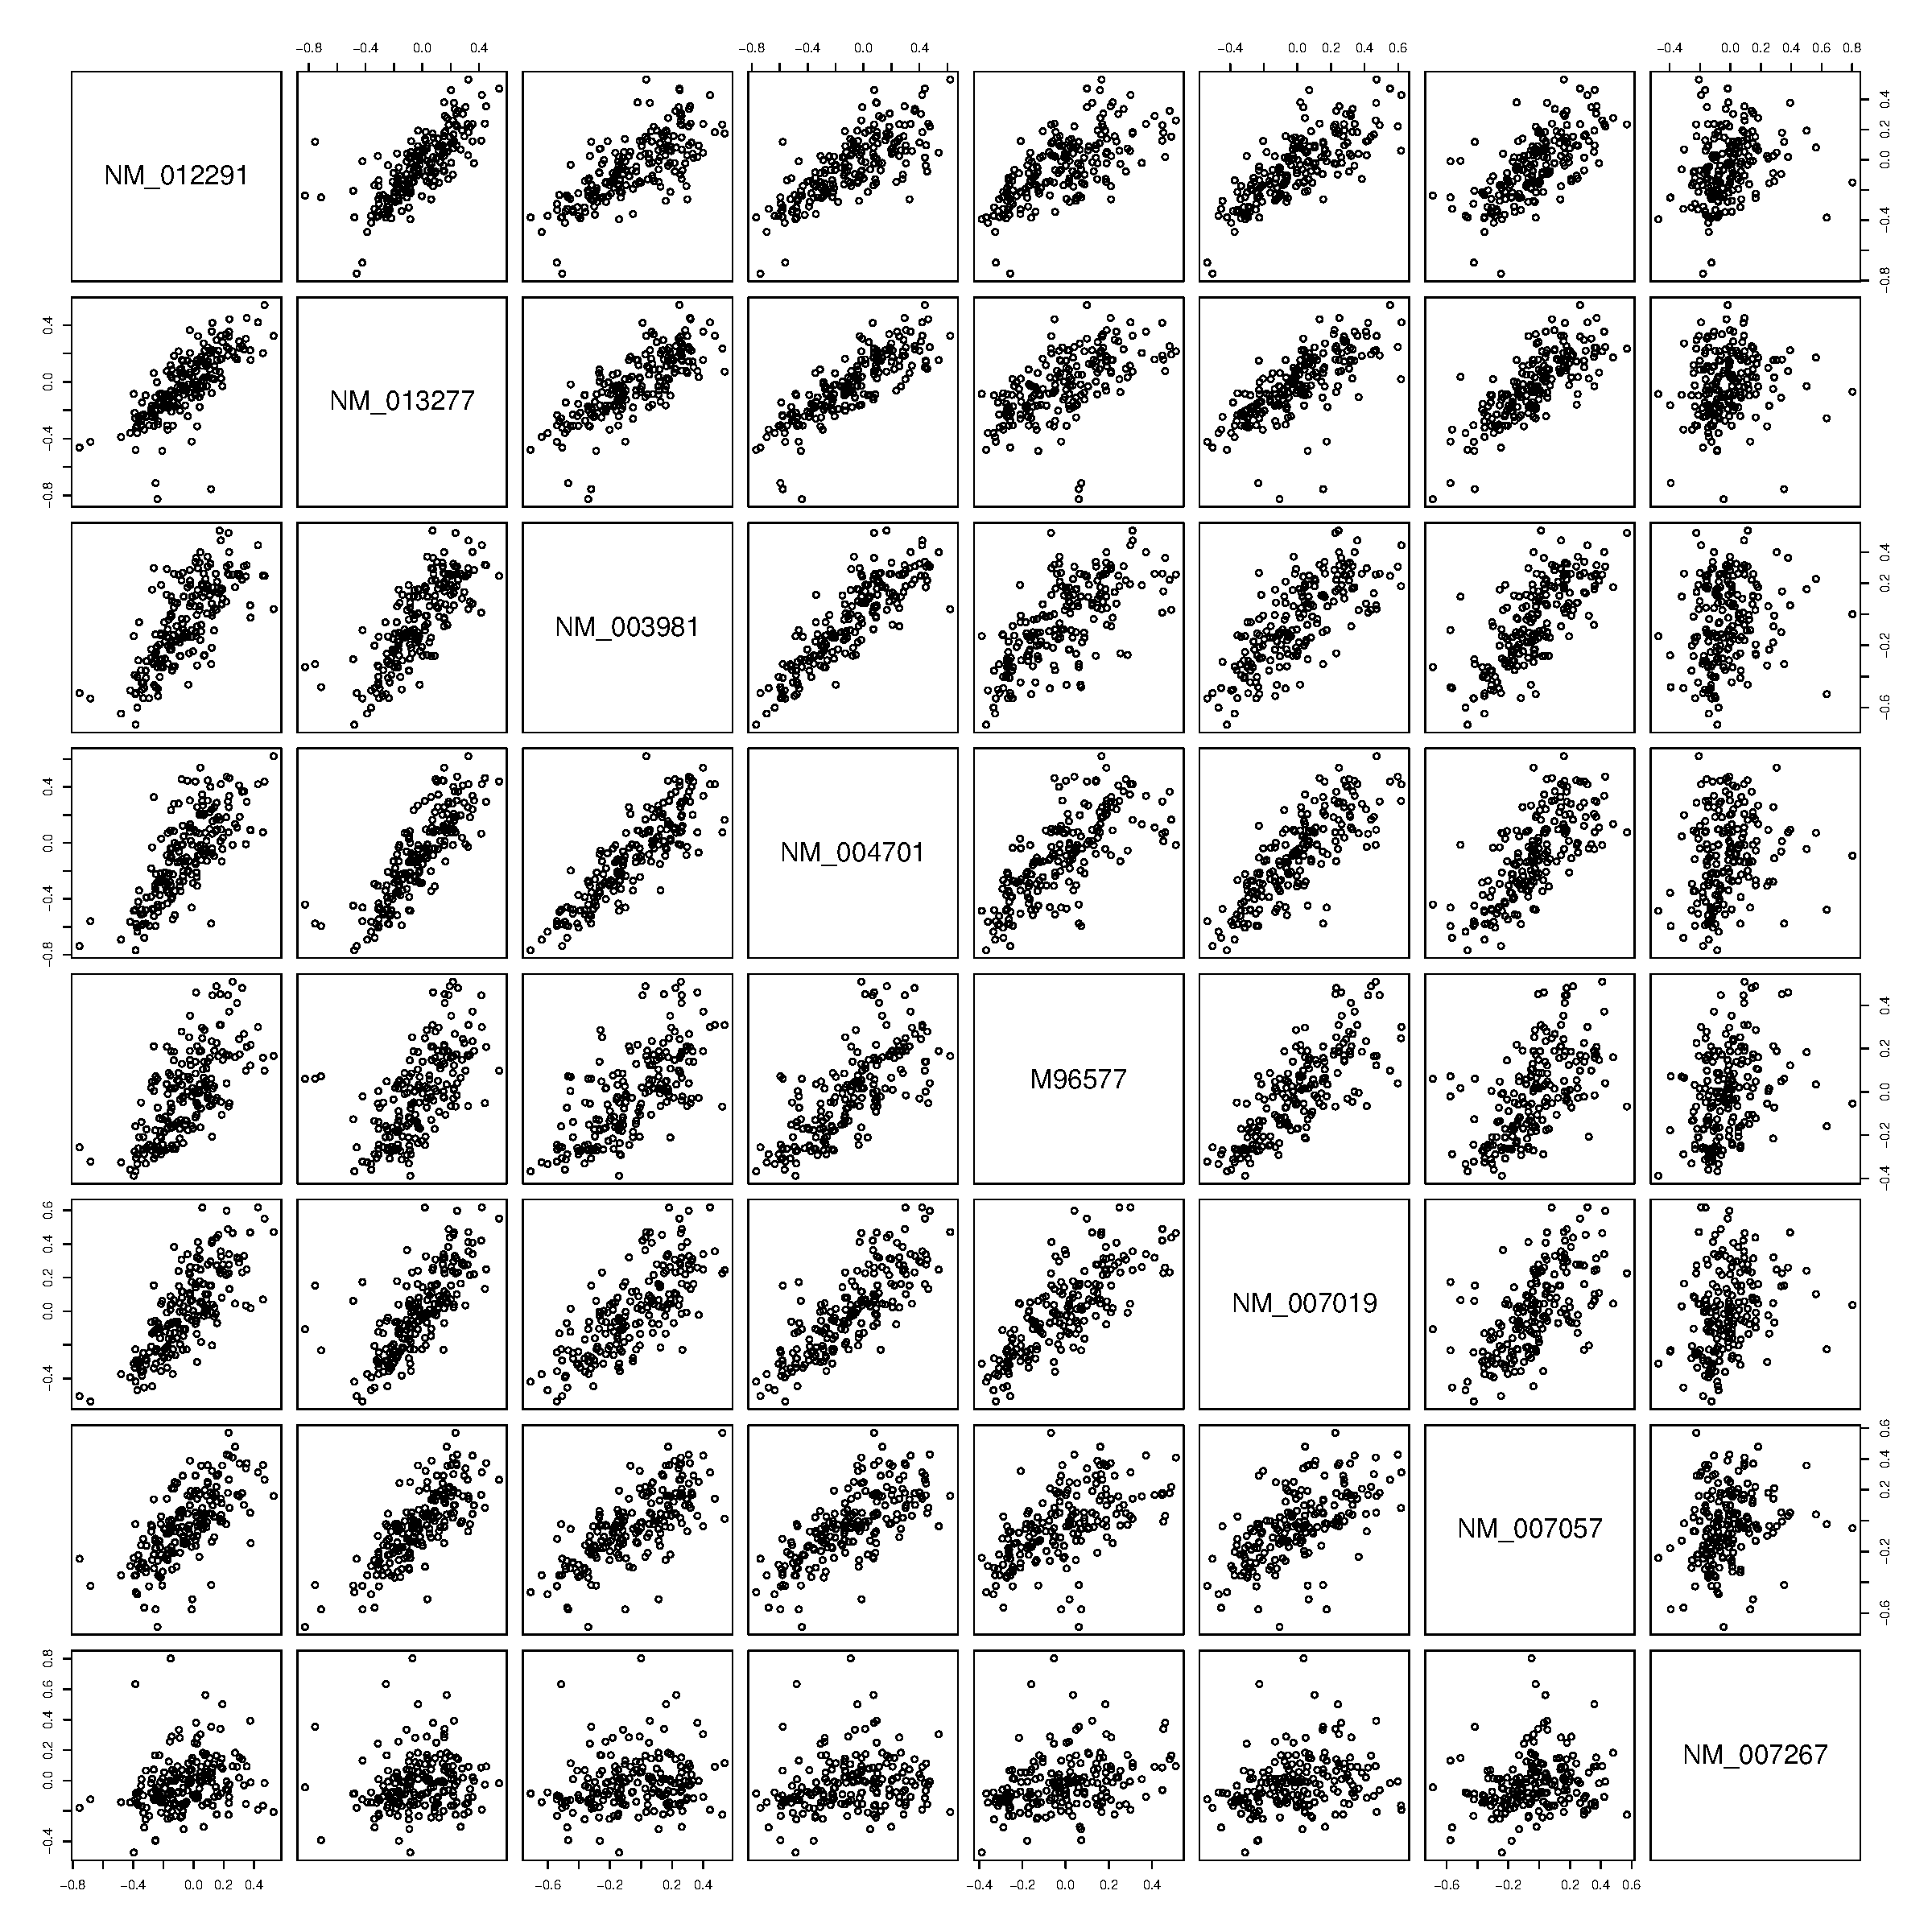
\includegraphics[scale=0.4]{pairs-colinearity.pdf}

\end{document}
